\ifx\wholebook\relax \else
\documentclass[b5paper]{article}
\usepackage[nomarginpar
  %, margin=.5in
]{geometry}

\addtolength{\oddsidemargin}{-0.05in}
\addtolength{\evensidemargin}{-0.05in}
\addtolength{\textwidth}{0.1in}
\usepackage[en]{../../../prelude}

\setcounter{page}{1}

\begin{document}

\title{Queue}

\author{Xinyu~LIU
\thanks{{\bfseries Xinyu LIU} \newline
  Email: liuxinyu95@gmail.com \newline}
  }

\maketitle
\fi

\markboth{Queue}{Elementary Algorithms}

\ifx\wholebook\relax
\chapter{Queue}
\numberwithin{Exercise}{chapter}
\fi

\section{Introduction}
\label{introduction}

Queue supports first-in, first-out (FIFO). There are many ways to implement queue, e.g., through linked list, doubly liked list, circular buffer, etc. Okasaki gave 16 different implementations in \cite{okasaki-book}. A queue satisfies the following two requirements:

\begin{enumerate}
\item Add a new element to the tail in constant time;
\item Access or remove an element from head in constant time.
\end{enumerate}

It's easy to realize queue with doubly linked list. We skip this implementation, and focus on using other basic data structures, like (singly) linked list or array.

\section{Linked-list queue}
\index{Queue!linked-list}

We can insert or remove element from the head of a linked list. However, to support FIFO, we have to do one operation in head, and the other in tail. We need $O(n)$ time traverse to reach the tail, where $n$ is the length. To achieve the constant time performance goal, we use an extra variable to record the tail position, and apply a sentinel node $S$ to simplify the empty queue case handling, as shown in figure \ref{fig:empty-list}.

\lstset{frame = single}
\begin{lstlisting}[language = Bourbaki]
data Node<K> {
  Key key
  Node next
}

data Queue {
  Node head, tail
}
\end{lstlisting}

\begin{figure}[htbp]
  \centering
  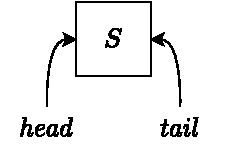
\includegraphics[scale=0.6]{img/empty-list}
  \caption{Both head and tail point to $S$ for empty queue.}
  \label{fig:empty-list}
\end{figure}

The two important queue operations are `enqueue' (also called push, snoc, append, or push back) and `dequeue' (also called pop, or pop front). When implement queue with list, we push on head, and pop from tail.

\begin{algorithmic}[1]
\Function{Enqueue}{$Q, x$}
  \State $p \gets $ \Call{Node}{$x$}
  \State \Call{Next}{$p$} $\gets$ NIL
  \State \textproc{Next}(\Call{Tail}{$Q$}) $\gets p$
  \State \Call{Tail}{$Q$} $\gets p$
\EndFunction
\end{algorithmic}

As there is at least a $S$ node even for empty queue, we need not check if the tail is NIL.

\begin{algorithmic}[1]
\Function{Dequeue}{$Q$}
  \State $x \gets $ \Call{Head}{$Q$}
  \State \textproc{Next}(\Call{Head}{$Q$}) $\gets$ \Call{Next}{$x$}
  \If{$x = $ \Call{Tail}{$Q$}} \Comment{$Q$ is empty}
    \State \Call{Tail}{$Q$} $\gets$ \Call{Head}{$Q$}
  \EndIf
  \State \Return \Call{Key}{$x$}
\EndFunction
\end{algorithmic}

As the $S$ node is ahead of all other nodes, \textproc{Head} actually returns the next node to $S$, as shown in figure \ref{fig:list-queue}. It's easy to expand this implementation to concurrent environment with two locks on the head and tail respectively. $S$ node helps to prevent dead-lock when the queue is empty\cite{PODC96}\cite{SutterDDJ}.

\begin{figure}[htbp]
  \centering
  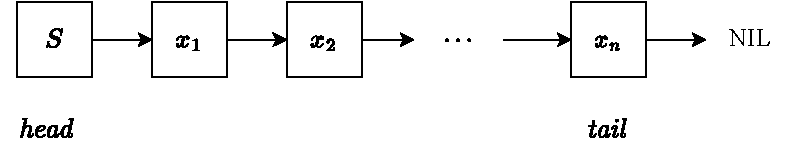
\includegraphics[scale=0.8]{img/slistq}
  \caption{List with $S$ node.}
  \label{fig:list-queue}
\end{figure}

\section{Circular buffer}
\index{Queue!Circular buffer}

Symmetrically, we can append element to the tail of array, but it takes linear time $O(n)$ to remove element from head. This is because we need shift all elements one cell ahead. The idea of circular buffer is to reuse the free cells before the first valid element after we remove elements from head, as shown figure \ref{fig:circular-buffer-queue}, and \ref{fig:circular-buffer}. We can use the head index, the length count, and the size of the array to define a queue. It's empty when the count is 0, it's full when count = size, we can also simplify the enqueue/dequeue implementation with modular operation.

\begin{figure}[htbp]
 \centering
 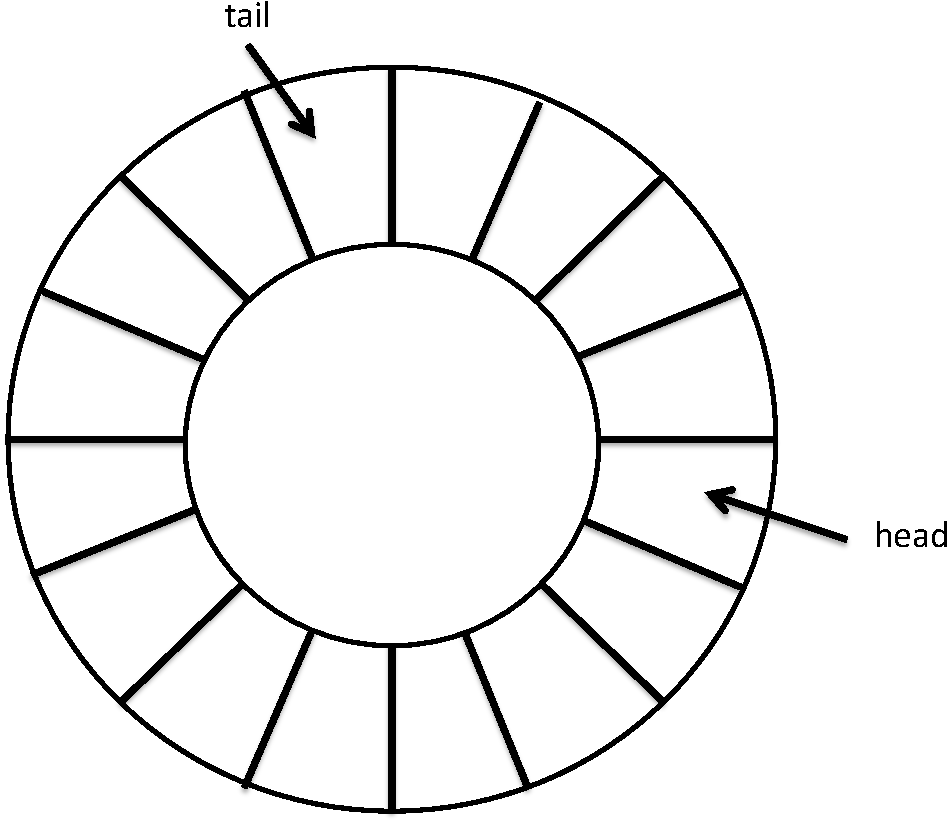
\includegraphics[scale=0.3]{img/ring-buffer}
 \caption{Circular buffer.}
 \label{fig:circular-buffer}
\end{figure}

\begin{figure}[htbp]
 \centering
 \subcaptionbox{Enqueue some elements.}{
 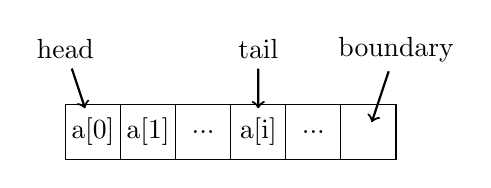
\begin{tikzpicture}[scale=0.7]
    \draw (0, 0) rectangle (1, 1) node (a0) [pos=.5] {a[0]}
          (1, 0) rectangle (2, 1) node [pos=.5] {a[1]}
          (2, 0) rectangle (3, 1) node [pos=.5] {...}
          (3, 0) rectangle (4, 1) node [pos=.5] (ai) {a[i]}
          (4, 0) rectangle (5, 1) node [pos=.5] {...}
          (5, 0) rectangle (6, 1) node (an) [pos=.5] {};
    \draw (0, 2) node (hd) {head}
          (3.5, 2) node (tl) {tail}
          (6, 2) node (bd) {boundary};
    \draw[thick, ->] (hd) edge (a0)
                 (tl) edge (ai)
                 (bd) edge (an);
  \end{tikzpicture}}
 \subcaptionbox{Free cells after dequeue.}{
  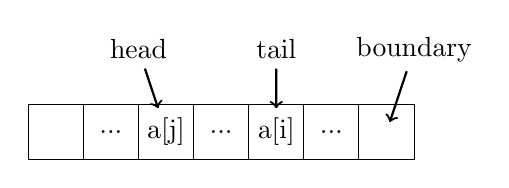
\begin{tikzpicture}[scale=0.7]
    \draw (0, 0) rectangle (1, 1)
          (1, 0) rectangle (2, 1) node [pos=.5] {...}
          (2, 0) rectangle (3, 1) node (aj) [pos=.5] {a[j]}
          (3, 0) rectangle (4, 1) node [pos=.5] {...}
          (4, 0) rectangle (5, 1) node (ai) [pos=.5] {a[i]}
          (5, 0) rectangle (6, 1) node [pos=.5] {...}
          (6, 0) rectangle (7, 1) node (an) [pos=.5] {};
    \draw (2, 2) node (hd) {head}
          (4.5, 2) node (tl) {tail}
          (7, 2) node (bd) {boundary};
    \draw[thick, ->] (hd) edge (aj)
                 (tl) edge (ai)
                 (bd) edge (an);
  \end{tikzpicture}} \\
 \subcaptionbox{Enqueue more elements to the boundary}{
   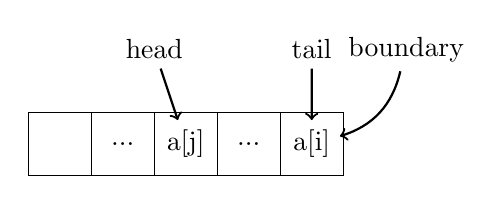
\begin{tikzpicture}[scale=0.8]
    \draw (0, 0) rectangle (1, 1)
          (1, 0) rectangle (2, 1) node [pos=.5] {...}
          (2, 0) rectangle (3, 1) node (aj) [pos=.5] {a[j]}
          (3, 0) rectangle (4, 1) node [pos=.5] {...}
          (4, 0) rectangle (5, 1) node (ai) [pos=.5] {a[i]};
    \draw (2, 2) node (hd) {head}
          (4.5, 2) node (tl) {tail}
          (6, 2) node (bd) {boundary};
    \draw[thick, ->] (hd) edge (aj)
                 (tl) edge (ai)
                 (bd) edge [bend left] (ai);
  \end{tikzpicture}}
 \subcaptionbox{Enqueue the next element to the first cell.}{
    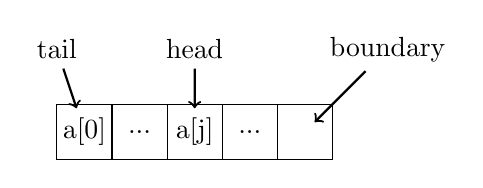
\begin{tikzpicture}[scale=0.7]
    \draw (0, 0) rectangle (1, 1) node (a0) [pos=.5] {a[0]}
          (1, 0) rectangle (2, 1) node [pos=.5] {...}
          (2, 0) rectangle (3, 1) node (aj) [pos=.5] {a[j]}
          (3, 0) rectangle (4, 1) node [pos=.5] {...}
          (4, 0) rectangle (5, 1) node (an) [pos=.5] {};
    \draw (2.5, 2) node (hd) {head}
          (0, 2) node (tl) {tail}
          (6, 2) node (bd) {boundary};
    \draw[thick, ->] (hd) edge (aj)
                 (tl) edge (a0)
                 (bd) edge (an);
  \end{tikzpicture}} \\
 \subcaptionbox{All cells are occupied, full.}{
   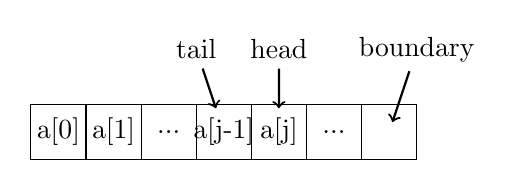
\begin{tikzpicture}[scale=0.7]
    \draw (0, 0) rectangle (1, 1) node [pos=.5] {a[0]}
          (1, 0) rectangle (2, 1) node [pos=.5] {a[1]}
          (2, 0) rectangle (3, 1) node [pos=.5] {...}
          (3, 0) rectangle (4, 1) node (a1j) [pos=.5] {a[j-1]}
          (4, 0) rectangle (5, 1) node (aj) [pos=.5] {a[j]}
          (5, 0) rectangle (6, 1) node [pos=.5] {...}
          (6, 0) rectangle (7, 1) node (an) [pos=.5] {};
    \draw (4.5, 2) node (hd) {head}
          (3, 2) node (tl) {tail}
          (7, 2) node (bd) {boundary};
    \draw[thick, ->] (hd) edge (aj)
                 (tl) edge (a1j)
                 (bd) edge (an);
  \end{tikzpicture}}
 \caption{Circular buffer queue}
 \label{fig:circular-buffer-queue}
\end{figure}

\begin{algorithmic}[1]
\Function{Enqueue}{$Q, x$}
  \If{not \Call{Full}{$Q$}}
    \State \Call{Count}{$Q$} $\gets$ \Call{Count}{$Q$} + 1
    \State tail $\gets $ (\Call{Head}{$Q$} + \Call{Count}{$Q$}) $\bmod$ \Call{Size}{$Q$}
    \State \Call{Buf}{$Q$}[tail] $\gets x$
  \EndIf
\EndFunction
\end{algorithmic}

\begin{algorithmic}[1]
\Function{Dequeue}{$Q$}
  \State $x \gets$ NIL
  \If{not \Call{Empty}{$Q$}}
    \State $h \gets$ \Call{Head}{$Q$}
    \State $x \gets$ \Call{Buf}{$Q$}[$h$]
    \State \Call{Head}{$Q$} $\gets $ (h + 1) $\bmod$ \Call{Size}{$Q$}
    \State \Call{Count}{$Q$} $\gets$ \Call{Count}{$Q$} - 1
  \EndIf
  \State \Return $x$
\EndFunction
\end{algorithmic}

\begin{Exercise}
The circular buffer is allocated with a predefined size. We can use two references head and tail instead of count. How to determine if a circular buffer queue is full or empty? (the head can be either ahead of tail or behind it.)
\end{Exercise}

\section{Paired-list queue}
\index{Queue!Paired-list queue}

We can access list head in constant time, but need linear time to access the tail. We can connect two lists `tail to tail' to implement queue, as shown in figure \ref{fig:horseshoe-magnet}. We define such queue as $(f, r)$, where $f$ is the front list, and $r$ is the rear list. The empty list is $([\ ], [\ ])$. We push new element to the head of $r$, and pop from the tail of $f$. Both are constant time.

\begin{figure}[htbp]
  \centering
  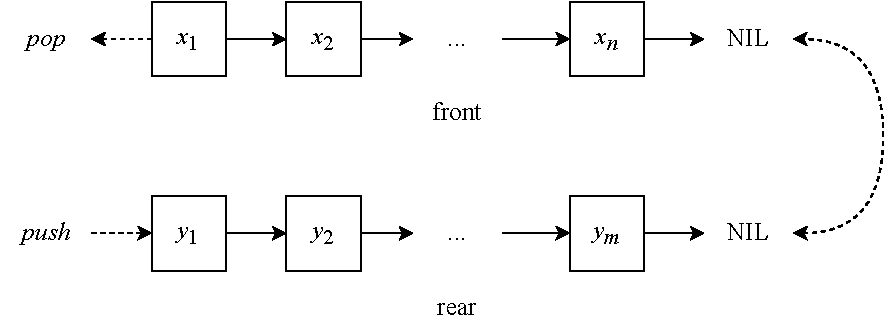
\includegraphics[scale=0.6]{img/paired-listq}
  \caption{paired-list queue.}
  \label{fig:horseshoe-magnet}
\end{figure}

\be
\begin{cases}
push\ x\ (f, r) & = (f, x \cons r) \\
pop\ (x \cons f, r)   & = (f, r) \\
\end{cases}
\ee

$f$ may become empty after a series of pops, while $r$ still contains elements. To continue pop, we reverse $r$ to replace $f$, i.e., $([\ ], r) \mapsto (reverse\ r, [\ ])$. We need check and adjust balance after every push/pop:

\be
\begin{array}{rcl}
\textit{balance}\ [\ ]\ r & = & (\textit{reverse}\ r, [\ ]) \\
\textit{balance}\ f\ r & = & (f, r) \\
\end{array}
\ee

Although the time is bound to linear time when reverse $r$, the amortised performance is constant time. We adjust the push/pop as below:

\be
\begin{cases}
push\ x\ (f, r) & = \textit{balance}\ f\ (x \cons r) \\
pop\ (x \cons f, r)   & = \textit{balance}\ f\ r \\
\end{cases}
\ee

\index{Queue!Paired-array queue}

There is a symmetric implementation with a pair of arrays. Table \ref{tab:array-list-comp} shows the symmetric between list and array. We connect two arrays head to head to form a queue, as shown in figure \ref{fig:horseshoe-array}. When array $R$ becomes empty, we reverse array $F$ to replace $R$.

\begin{table}[htbp]
\centering
\begin{tabular}{l | c | r}
  \hline
  operation & array & list \\
  \hline
  insert to head & $O(n)$ & $O(1)$ \\
  append to tail & $O(1)$ & $O(n)$ \\
  remove from head & $O(n)$ & $O(1)$ \\
  remove from tail & $O(1)$ & $O(n)$ \\
  \hline
\end{tabular}
\caption{array and list}
\label{tab:array-list-comp}
\end{table}

\begin{figure}[htbp]
  \centering
  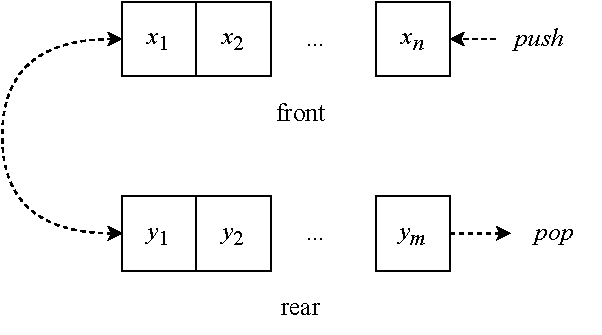
\includegraphics[scale=0.6]{img/paired-arrayq}
  \caption{paired-array queue.}
  \label{fig:horseshoe-array}
\end{figure}

\begin{Exercise}
\Question{Why need balance check and adjustment after push?}
\Question{Prove the amortized performance of paired-list queue is constant time.}
\Question{Implement the paired-array queue.}
\end{Exercise}

\begin{Answer}
\Question{Why need balance check and adjustment after push?

Consider the case, first $push\ a\ ([\ ], [\ ])$, then $pop$.
}
\Question{Prove the amortized performance of paired-list queue is constant time.}
\Question{Implement the paired-array queue.

\begin{algorithmic}[1]
\Function{Push}{$Q, x$}
  \State \textproc{Append}(\Call{Front}{$Q$}, $x$)
\EndFunction
\Statex
\Function{Pop}{$Q$}
  \If{\Call{Rear}{$Q$} $= [\ ]$}
    \State \Call{Rear}{$Q$} $\gets$ \textproc{Reverse}(\Call{Front}{$Q$})
    \State \Call{Front}{$Q$} $\gets [\ ]$
  \EndIf
  \State $n \gets$ \textproc{Length}(\Call{Rear}{$Q$})
  \State $x \gets$ \Call{Rear}{$Q$}[n]
  \State \textproc{Length}(\Call{Rear}{$Q$}) $\gets n - 1$
  \State \Return $x$
\EndFunction
\end{algorithmic}
}
\end{Answer}

\section{Balance Queue}
\index{Queue!Balance Queue}

Although paired-list queue performs in amortized constant time, it is linear time in worse case. For e.g., there is an element in $f$, then repeat pushing $n$ elements. Now it takes $O(n)$ time to pop. The lengths of $f$ and $r$ are unbalance in this case. To solve it, we add another rule: keep the length of $r$ is not greater than $f$, otherwise we reverse.

\be
  |r| \leq |f|
\label{eq:balance-invariant}
\ee

We check the lengths in every push/pop, however, it takes linear time to compute length. We can record the length in a variable, and update it during push/pop. Denote the paired-list queue as $(f, n, r, m)$, where $n = |f|$, $m = |r|$. From the balance rule (\ref{eq:balance-invariant}), we can check the length of $f$ to test if a queue is empty:

\be
  Q = \phi \iff n = 0
\ee

The definition of push/pop change to:

\be
\begin{cases}
  push\ x\ (f, n, r, m) & = \textit{balance}\ (f, n,  x \cons r, m + 1) \\
  pop\ (x \cons f, n, r, m) & = \textit{balance}\ (f, n - 1, r, m) \\
\end{cases}
\ee

Where \textit{balance} is defined as:

\be
\textit{balance}\ (f, n, r, m) = \begin{cases}
  m \leq n: & (f, n, r, m) \\
  \text{otherwise}: & (f \doubleplus reverse\ r, m + n, [\ ], 0)\\
\end{cases}
\ee

\section{Real-time queue}
\index{Queue!Real-time queue}

It still takes linear time to reverse, concatenate lists in balanced queue. A real-time queue need guarantee constant time in every push/pop operation. The performance bottleneck happens in $f \doubleplus reverse\ r$. At this time, $m > $, breaks the balance rule. Since $m, n$ are integers, we know $m = n + 1$. $\doubleplus$ takes $O(n)$ time, and reverse takes $O(m)$ time. The total time is bound to $O(n + m)$, which is proportion to the number of elements. Our solution is to distribute this computation to multiple push and pop operations. Let's revisit the tail recursive\cite{wiki-tail-call}\cite{recursion} reverse:

\be
reverse\ = reverse'\ [\ ]
\ee

This is in Curried form, where:

\be
\begin{array}{rcl}
\textit{reverse}'\ a\ [\ ] & = & a \\
\textit{reverse}'\ a\ (x \cons xs) & = & \textit{reverse}'\ (x \cons a)\ xs \\
\end{array}
\ee

We can turn the tail recursive implementation to stepped computation. We model it as a series of state transformation. Define a state machine with two states: reverse state $S_r$, and complete state $S_f$. We {\em slow-down} the reverse computation as below:

\be
\begin{array}{rcl}
step\ S_r\ a\ [\ ] & = & (S_f, a) \\
step\ S_r\ a\ (x \cons xs) & = & (S_r, (x \cons a), xs) \\
\end{array}
\ee

Each step, we check and transform the state. $S_r$ means the reverse is on going. If there is no remaining element to reverse, we change the state to $S_f$ (done); otherwise, we pick the head element $x$, link it ahead of $a$. This step terminates, but not continues to recursion. The new state with the intermediate reverse result will be input to the next $step$. For example:

\[
\begin{array}{rcl}
step\ S_r\ \text{``hello''}\ [\ ] & = & (S_r, \text{``ello''}, \text{``h''}) \\
step\ S_r\ \text{``ello''}\ \text{``h''} & = & (S_r, \text{``llo''}, \text{``eh''}) \\
... & & \\
step\ S_r\ \text{``o''}\ \text{``lleh''} & = & (S_r, [\ ], \text{``olleh''}) \\
step\ S_r\ [\ ]\ \text{``olleh''} & = & (S_f, \text{``olleh''})
\end{array}
\]

We can next distribute the reverse steps to push/pop operations. However, it only solves half problem. We next need slow-down $\doubleplus$ computation, which is more complex. We use state machine too. To concatenate $xs \doubleplus ys$, we first reverse $xs$ to $\overleftarrow{xs}$, then pick elements form $\overleftarrow{xs}$ one by one, and link each head of $ys$. The idea is similar to $\textit{reverse}'$:

\be
  \begin{array}{rcl}
    xs \doubleplus ys & = & (reverse\ reverse\ xs) \doubleplus ys \\
             & = & (reverse'\ [\ ]\ (reverse\ xs)) \doubleplus ys \\
             & = & reverse'\ ys\ (reverse\ xs) \\
             & = & reverse'\ ys\ \overleftarrow{xs}
  \end{array}
\ee

We need add another state. After reverse $r$, we step by step concatenate from $\overleftarrow{f}$. The three states are: $S_r$ of reverse, $S_c$ of concatenate, $S_f$ of completion. The two phases are:

\begin{enumerate}
\item Reverse $f$ and $r$ in parallel to: $\overleftarrow{f}$ and
$\overleftarrow{r}$ step by step;
\item Stepped taking elements from $\overleftarrow{f}$, and link each ahead of $\overleftarrow{r}$.
\end{enumerate}

\be
\begin{array}{rcll}
next\ (S_r, f', x \cons f, r', y \cons r) & = & (S_r, x \cons f', f, y \cons r', r) & \text{stepped reverse}\ f, r\\
next\ (S_r, f', [\ ], r', [y]) & = & next\ (S_c, f', y \cons r') & \text{reverse done, start to concatenate}\\
next\ (S_c, a, [\ ]) & = & (S_f, a) & \text{concatenate done}\\
next\ (S_c, a, x \cons f') & = & (S_c, x \cons a, f') & \text{stepped concatenate}\\
\end{array}
\ee

All left to us is to distribute these incremental steps into every pop and push
operations to implement a real-time $O(1)$ purely functional queue.

Before we dive into the final real-time queue implementation, let's analyze how
many incremental steps are taken to achieve the result of $F \cup reverse(R)$.
According to the balance variant we used previously, $|R| = |F| + 1$, Let's
denotes $m = |F|$.

Once the queue gets unbalanced due to some push or pop operation, we start this
incremental  $F \cup reverse(R)$.
It needs $m + 1$ steps to reverse $R$, and at the same time, we finish reversing
the list $F$ within these steps. After that, we need extra $m+1$ steps to execute
the concatenation. So there are $2m + 2$ steps.

It seems that distribute one step inside one pop or push operation is the natural
solution. However, there is a critical
question must be answered: Is it possible that before we finish these $2m + 2$ steps,
the queue gets unbalanced again due to a series push and pop?

There are two facts about this question, one is good news and the other is bad news.

Let's first show the good news, that luckily, continuously pushing can't make the
queue unbalanced again before we finish these $2m + 2$ steps to achieve $F \cup reverse(R)$.
This is because once we start re-balancing, we can get a new front list
$F' = F \cup reverse(R)$ after $2m + 2$ steps. While the next time unbalance
is triggered when

\be
  \begin{array}{rcl}
  |R'| & = & |F'| + 1 \\
       & = & |F| + |R| + 1 \\
       & = & 2m + 2
  \end{array}
\ee

That is to say, even we continuously pushing as mush elements as possible after
the last unbalanced time, when the queue gets unbalanced again, the $2m+2$ steps
exactly get finished at that time point. Which means the new front list $F'$ is
calculated OK. We can safely go on to compute $F' \cup reverse(R')$. Thanks to the
balance invariant which is designed in previous section.

But, the bad news is that, pop operation can happen at anytime before these
$2m+2$ steps finish. The situation is that once we want to extract element
from front list, the new front list $F' = F \cup reverse(R)$ hasn't been
ready yet. We don't have a valid front list at hand.

One solution to this problem is to keep a copy of original front list $F$,
during the time we are calculating $reverse(F)$ which is described in phase 1 of
our incremental computing strategy. So that we are still safe even if user
continuously performs first $m$ pop operations. So the queue looks like
in table \ref{tab:pop-before-m} at some time after we start the incremental computation and before
phase 1 (reverse $F$ and $R$ simultaneously) ending\footnote{One may wonder that copying
a list takes linear time to the length of the list. If so the whole solution
would make no sense. Actually, this linear time copying won't happen at all.
This is because the purely functional nature, the front list won't be mutated
either by popping or by reversing. However, if trying to realize a symmetric
solution with paired-array and mutate the array in-place, this issue should be stated, and
we can perform a `lazy' copying, that the real copying
work won't execute immediately, instead, it copies one element every step we
do incremental reversing. The detailed implementation is left as an exercise.}.

\begin{table}
\centering
\begin{tabular}{l l l}
  front copy & on-going computation & new rear \\
  \hline
  $\{ f_i, f_{i+1}, ..., f_M \}$ & $(S_r, \tilde{F}, ..., \tilde{R}, ...)$ & $ \{ ... \}$ \\
  first $i-1$ elements popped & intermediate result $\overleftarrow{F}$ and $\overleftarrow{R}$ & new elements pushed
\end{tabular}
\caption{Intermediate state of a queue before first $m$ steps finish.}
\label{tab:pop-before-m}
\end{table}

After these $M$ pop operations, the copy of $F$ is exhausted. And we just
start incremental concatenation phase at that time. What if user goes
on popping?

The fact is that since $F$ is exhausted (becomes $\phi$), we needn't do concatenation
at all. Since $F \cup \overleftarrow{R} = \phi \cup \overleftarrow{R} = \overleftarrow{R}$.

It indicates us, when doing concatenation, we only need to concatenate those elements
haven't been popped, which are still left in $F$. As user pops elements one by one
continuously from the head of front list $F$, one method is to use a counter,
record how many elements there are still in $F$. The counter is initialized as 0
when we start computing $F \cup reverse(R)$, it's increased by one when we reverse
one element in $F$, which means we need concatenate this element in the future;
and it's decreased by one every time when pop is
performed, which means we can concatenate one element less; of course we need decrease
this counter as well in every steps of concatenation. If and only if this counter
becomes zero, we needn't do concatenations any more.

We can give the realization of purely functional real-time queue according to the above
analysis.

We first add an idle state $S_0$ to simplify some state transferring. Below Haskell program
is an example of this modified state definition.

\lstset{language=Haskell}
\begin{lstlisting}
data State a = Empty
             | Reverse Int [a] [a] [a] [a] -- n, f', acc\_f' r, acc\_r
             | Append Int [a] [a]          -- n, rev\_f', acc
             | Done [a] -- result: f ++ reverse r
\end{lstlisting}

And the data structure is defined with three parts, the front list (augmented with length);
the on-going state of computing $F \cup reverse(R)$; and the rear list (augmented with length).

Here is the Haskell definition of real-time queue.

\lstset{language=Haskell}
\begin{lstlisting}
data RealtimeQueue a = RTQ [a] Int (State a) [a] Int
\end{lstlisting}

The empty queue is composed with empty front and rear list together with idle state $S_0$ as
$Queue(\phi, 0, S_0, \phi, 0)$. And we can test if a queue is empty by checking if $|F| = 0$
according
to the balance invariant defined before. Push and pop are changed accordingly.

\be
  push(Q, x) = balance(F, |F|, \mathcal{S}, \{ x \} \cup R, |R|+1)
\ee

\be
  pop(Q) = balance(F', |F|-1, abort(\mathcal{S}), R, |R|)
\ee

The major difference is $abort()$ function. Based on our above analysis, when there
is popping, we need decrease the counter, so that we can concatenate one element less.
We define this as aborting. The details will be given after $balance()$ function.

The relative Haskell code for push and pop are listed like this.

\lstset{language=Haskell}
\begin{lstlisting}
push (RTQ f lenf s r lenr) x = balance f lenf s (x:r) (lenr + 1)
pop (RTQ (_:f) lenf s r lenr) = balance f (lenf - 1) (abort s) r lenr
\end{lstlisting}

The $balance()$ function first check the balance invariant, if it's violated, we need
start re-balance it by starting compute $F \cup reverse(R)$ incrementally; otherwise
we just execute one step of the unfinished incremental computation.

\be
  balance(F, |F|, \mathcal{S}, R, |R|) = \left \{
  \begin{array}
  {r@{\quad:\quad}l}
  step(F, |F|, \mathcal{S}, R, |R|) & |R| \leq |F| \\
  step(F, |F| + |R|, (S_r, 0, F, \phi, R, \phi) \phi, 0) & otherwise
  \end{array}
\right .
\ee

The relative Haskell code is given like below.

\lstset{language=Haskell}
\begin{lstlisting}
balance f lenf s r lenr
    | lenr <= lenf =  step f lenf s r lenr
    | otherwise = step f (lenf + lenr) (Reverse 0 f [] r []) [] 0
\end{lstlisting}

The $step()$ function typically transfer the state machine one state ahead, and
it will turn the state to idle ($S_0$) when the incremental computation finishes.

\be
  step(F, |F|, \mathcal{S}, R, |R|) = \left \{
  \begin{array}
  {r@{\quad:\quad}l}
  Queue(F', |F|, S_0, R, |R|) &  S' = S_f \\
  Queue(F, |F|, \mathcal{S}', R, |R|) & otherwise
  \end{array}
  \right .
\ee

Where $\mathcal{S}' = next(\mathcal{S})$ is the next state transferred;
$F' = F \cup reverse(R)$, is the final new front list result from the incremental
computing. The real
state transferring is implemented in $next()$ function as the following. It's different
from previous version by adding the counter field $n$ to record how many elements left
we need to concatenate.

\be
  next(\mathcal{S}) = \left \{
  \begin{array}
  {r@{\quad:\quad}l}
  (S_r, n+1, F', \{ f_1 \} \cup \overleftarrow{F}, R', \{ r_1 \} \cup \overleftarrow{R}) &
      S = S_r \land F \neq \phi \\
  (S_c, n, \overleftarrow{F}, \{ r_1 \} \cup \overleftarrow{R}) &
      S = S_r \land F = \phi \\
  (S_f, A) & S = S_c \land n = 0 \\
  (S_c, n-1, X', \{ x_1 \} \cup A) & S = S_c \land n \neq 0 \\
  \mathcal{S} & otherwise
  \end{array}
\right .
\ee

And the corresponding Haskell code is like this.

\lstset{language=Haskell}
\begin{lstlisting}
next (Reverse n (x:f) f' (y:r) r') = Reverse (n+1) f (x:f') r (y:r')
next (Reverse n [] f' [y] r') = Concat n f' (y:r')
next (Concat 0 _ acc) = Done acc
next (Concat n (x:f') acc) = Concat (n-1) f' (x:acc)
next s = s
\end{lstlisting}

Function $abort()$ is used to tell the state machine, we can concatenate one element
less since it is popped.

\be
  abort(\mathcal{S}) = \left \{
  \begin{array}
  {r@{\quad:\quad}l}
  (S_f, A') & S = S_c \land n = 0 \\
  (S_c, n-1, X' A) & S = S_c \land n \neq 0 \\
  (S_r, n-1, F, \overleftarrow{F}, R, \overleftarrow{R}) & S = S_r \\
  \mathcal{S} & otherwise
  \end{array}
\right .
\ee

Note that when $n = 0$ we actually rollback one concatenated element by
return $A'$ as the result but not $A$. (Why? this is left as an exercise.)

The Haskell code for abort function is like the following.

\lstset{language=Haskell}
\begin{lstlisting}
abort (Concat 0 _ (_:acc)) = Done acc     -- Note! we rollback 1 elem
abort (Concat n f' acc) = Concat (n-1) f' acc
abort (Reverse n f f' r r') = Reverse (n-1) f f' r r'
abort s = s
\end{lstlisting}

It seems that we've done, however, there is still one tricky issue hidden
behind us.
If we push an element $x$ to an empty queue, the result queue will be:
\[
  Queue(\phi, 1, (S_c, 0, \phi, \{ x \}), \phi, 0)
\]

If we perform pop immediately, we'll get an error! We found that
the front list is empty although the previous computation of $F \cup reverse(R)$
has been finished. This is because it takes one more extra step to
transfer from the state $(S_c, 0, \phi, A)$ to $(S_f, A)$. It's necessary
to refine the $\mathcal{S}'$ in $step()$ function a bit.

\be
  \mathcal{S}' = \left \{
  \begin{array}
  {r@{\quad:\quad}l}
  next(next(\mathcal{S})) & F = \phi \\
  next(\mathcal{S}) & otherwise
  \end{array}
\right .
\ee

The modification reflects to the below Haskell code:

\lstset{language=Haskell}
\begin{lstlisting}
step f lenf s r lenr =
    case s' of
      Done f' -> RTQ f' lenf Empty r lenr
      s' -> RTQ f lenf s' r lenr
    where s' = if null f then next $ next s else next s
\end{lstlisting} %$

Note that this algorithm differs from the one given by Chris Okasaki in \cite{okasaki-book}.
Okasaki's algorithm executes two steps per pop and push, while the one presents in
this chapter executes only one per pop and push, which leads to more distributed
performance.

\begin{Exercise}
\begin{itemize}
\item Why need we rollback one element when $n=0$ in $abort()$ function?

\item Realize the real-time queue with symmetric paired-array queue solution in your favorite
imperative programming language.

\item In the footnote, we mentioned that when we start incremental reversing
with in-place paired-array solution, copying the array can't be done monolithic
or it will lead to linear time operation. Implement the lazy copying
so that we copy one element per step along with the reversing.

\end{itemize}
\end{Exercise}

\section{Lazy real-time queue}
\index{Queue!Lazy real-time queue}

The key to realize a real-time queue is to break down the expensive
$F \cup reverse(R)$ to avoid monolithic computation. Lazy evaluation
is particularly helpful in such case. In this section, we'll explore
if there is some more elegant solution by exploit laziness.

Suppose that there exits a function $rotate()$,
which can compute $F \cup reverse(R)$ incrementally. that's to say,
with some accumulator $A$, the following two functions are equivalent.

\be
  rotate(X, Y, A) \equiv X \cup reverse(Y) \cup A
  \label{eq:rot-def}
\ee

Where we initialized $X$ as the front list $F$, $Y$ as the rear list $R$,
and the accumulator $A$ is initialized as empty $\phi$.

The trigger of rotation is still as same as before when $|F| + 1 = |R|$.
Let's keep this constraint as an invariant during the whole rotation process,
that $|X| + 1 = |Y|$ always holds.

It's obvious to deduce to the trivial case:

\be
  rotate(\phi, \{ y_1 \}, A) = \{ y_1 \} \cup A
\ee

Denote $X = \{ x_1, x_2, ... \}$, $Y = \{ y_1, y_2, ...\}$, and
$X' = \{ x_2, x_3, ...  \}$, $Y' = \{ y_2, y_3, ...\}$ are the rest
of the lists without the first element for $X$ and $Y$ respectively.
The recursion case is ruled out as the following.

\be
  \begin{array}{rcll}
  rotate( X, Y, A ) & \equiv & X \cup reverse(Y) \cup A & \mbox{Definition of (}\ref{eq:rot-def} \mbox{)} \\
  & \equiv & \{ x_1 \} \cup (X' \cup reverse(Y) \cup A) & \mbox{Associative of } \cup \\
  & \equiv & \{ x_1 \} \cup (X' \cup reverse(Y') \cup (\{ y_1 \} \cup A)) & \mbox{Nature of reverse and associative of }  \cup \\
  & \equiv & \{ x_1 \} \cup rotate(X', Y', \{ y_1 \} \cup A) & \mbox{Definition of (} \ref{eq:rot-def} \mbox{)}
  \end{array}
\ee

Summarize the above two cases, yields the final incremental rotate algorithm.

\be
rotate(X, Y, A) = \left \{
  \begin{array}
  {r@{\quad:\quad}l}
  \{ y_1 \} \cup A & X = \phi \\
  \{ x_1 \} \cup rotate(X', Y', \{ y_1 \} \cup A) & otherwise
  \end{array}
\right .
\ee

If we execute $\cup$ lazily instead of strictly, that is, execute $\cup$
once pop or push operation is performed, the computation of $rotate$ can
be distribute to push and pop naturally.

Based on this idea, we modify the paired-list queue definition to change
the front list to a lazy list, and augment it with a computation stream.
\cite{SICP}. When the queue triggers re-balance constraint by some
pop/push, that
$|F| + 1 = |R|$, The algorithm creates a lazy rotation computation,
then use this lazy rotation as the new front list $F'$; the new rear
list becomes $\phi$, and a copy of $F'$ is maintained as a stream.

After that, when we performs every push and pop; we consume the
stream by forcing a $\cup$ operation. This results us advancing one
step along the stream, $ \{ x \} \cup F''$, where $F'' = tail(F')$.
We can discard $x$, and replace the stream $F'$ with $F''$.

Once all of the stream is exhausted, we can start another rotation.

In order to illustrate this idea clearly, we turns to Scheme/Lisp
programming language to show example codes, because it gives us
explicit control of laziness.

In Scheme/Lisp, we have the following three tools to deal with lazy
stream.

\lstset{language=Lisp}
\begin{lstlisting}
(define (cons-stream a b) (cons a (delay b)))

(define stream-car car)

(define (stream-cdr s) (cdr (force s)))
\end{lstlisting}

Function \texttt{cons-stream} constructs a 'lazy' list from an element $x$
and an existing list $L$ without really evaluating
the value of $L$; The evaluation is actually delayed to
\texttt{stream-cdr}, where the computation is forced. delaying can
be realized by lambda calculus as described in\cite{SICP}.

The lazy paired-list queue is defined as the following.

\lstset{language=Lisp}
\begin{lstlisting}
(define (make-queue f r s)
  (list f r s))

;; Auxiliary functions
(define (front-lst q) (car q))

(define (rear-lst q) (cadr q))

(define (rots q) (caddr q))
\end{lstlisting}

A queue is consist of three parts, a front list, a rear list,
and a stream which represents the computation of $F \cup reverse(R)$.
Create an empty queue is trivial as making all these three parts
null.

\begin{lstlisting}
(define empty (make-queue '() '() '()))
\end{lstlisting}

Note that the front-list is also lazy stream actually, so we need use
stream related functions to manipulate it. For example, the following
function test if the queue is empty by checking the front lazy list stream.

\begin{lstlisting}
(define (empty? q) (stream-null? (front-lst q)))
\end{lstlisting}

The push function is almost as same as the one given in previous section.
That we put the new element in front of the rear list; and then examine
the balance invariant and do necessary balancing works.

\be
push(Q, x) = balance(\mathcal{F}, \{ x \} \cup R, \mathcal{R}_s)
\ee

Where $\mathcal{F}$ represents the lazy stream of front list; $\mathcal{R}_s$ is
the stream of rotation computation. The relative Scheme/Lisp
code is give below.

\begin{lstlisting}
(define (push q x)
  (balance (front-lst q) (cons x (rear q)) (rots q)))
\end{lstlisting}

While pop is a bit different, because the front list is actually lazy stream,
we need force an evaluation. All the others are as same as before.

\be
pop(Q) = balance(\mathcal{F}', R, \mathcal{R}_s)
\ee

Here $\mathcal{F}'$, force one evaluation to $\mathcal{F}$, the Scheme/Lisp
code regarding to this equation is as the following.

\begin{lstlisting}
(define (pop q)
  (balance (stream-cdr (front-lst q)) (rear q) (rots q)))
\end{lstlisting}

For illustration purpose, we skip the error handling (such as pop from
an empty queue etc) here.

And one can access the top element in the queue by extract from
the front list stream.

\begin{lstlisting}
(define (front q) (stream-car (front-lst q)))
\end{lstlisting}

The balance function first checks if the computation stream is completely
exhausted, and starts new rotation accordingly; otherwise, it just consumes
one evaluation by enforcing the lazy stream.

\be
balance(Q) = \left \{
  \begin{array}
  {r@{\quad:\quad}l}
  Queue(\mathcal{F}', \phi, \mathcal{F}') & \mathcal{R}_s = \phi \\
  Queue(\mathcal{F}, R, \mathcal{R}_s') & otherwise
  \end{array}
\right .
\ee

Here $\mathcal{F}'$ is defined to start a new rotation.

\be
  \mathcal{F}' = rotate(F, R, \phi)
\ee

The relative Scheme/Lisp program is listed accordingly.

\begin{lstlisting}
(define (balance f r s)
  (if (stream-null? s)
      (let ((newf (rotate f r '())))
    (make-queue newf '() newf))
      (make-queue f r (stream-cdr s))))
\end{lstlisting}

The implementation of incremental rotate function is just as same as
what we analyzed above.

\begin{lstlisting}
(define (rotate xs ys acc)
  (if (stream-null? xs)
      (cons-stream (car ys) acc)
      (cons-stream (stream-car xs)
           (rotate (stream-cdr xs) (cdr ys)
               (cons-stream (car ys) acc)))))
\end{lstlisting}

We used explicit lazy evaluation in Scheme/Lisp. Actually, this program
can be very short by using lazy programming languages, for example,
Haskell.

\lstset{language=Haskell}
\begin{lstlisting}
data LazyRTQueue a = LQ [a] [a] [a] -- front, rear, f ++ reverse r

instance Queue LazyRTQueue where
    empty = LQ [] [] []

    isEmpty (LQ f _ _) = null f

    -- O(1) time push
    push (LQ f r rot) x = balance f (x:r) rot

    -- O(1) time pop
    pop (LQ (_:f) r rot) = balance f r rot

    front (LQ (x:_) _ _) = x

balance f r [] = let f' = rotate f r [] in LQ f' [] f'
balance f r (_:rot) = LQ f r rot

rotate [] [y] acc = y:acc
rotate (x:xs) (y:ys) acc = x : rotate xs ys (y:acc)
\end{lstlisting}

\section{Notes and short summary}
Just as mentioned in the beginning of this book in the first chapter,
queue isn't so simple as it was thought. We've tries to explain
algorithms and data structures both in imperative and in function
approaches; Sometimes, it gives impression that functional way is
simpler and more expressive in most time. However, there are still
plenty of areas, that more studies and works are needed to give equivalent
functional solution. Queue is such an important topic, that it
links to many fundamental purely functional data structures.

That's why Chris Okasaki made intensively study and took a great
amount of discussions in \cite{okasaki-book}. With purely functional
queue solved, we can easily implement dequeue with the similar
approach revealed in this chapter. As we can handle elements effectively
in both head and tail, we can advance one step ahead to realize
sequence data structures, which support fast concatenate, and
finally we can realize random access data structures to mimic
array in imperative settings. The details will be explained
in later chapters.

Note that, although we haven't mentioned priority queue, it's quite
possible to realized it with heaps. We have covered topic of heaps
in several previous chapters.

\begin{Exercise}
\begin{itemize}
\item Realize dequeue, which support adding and removing elements on both sides in
constant $O(1)$ time in purely functional way.
\item Realize dequeue in a symmetric solution only with array in your
favorite imperative programming language.
\end{itemize}
\end{Exercise}

\ifx\wholebook\relax \else
\section{Answers}
\shipoutAnswer

\begin{thebibliography}{99}

\bibitem{PODC96}
Maged M. Michael and Michael L. Scott. ``Simple, Fast, and Practical Non-Blocking and Blocking Concurrent Queue Algorithms''. \url{http://www.cs.rochester.edu/research/synchronization/pseudocode/queues.html}

\bibitem{SutterDDJ}
Herb Sutter. ``Writing a Generalized Concurrent Queue''. Dr. Dobb's Oct 29, 2008. \url{http://drdobbs.com/cpp/211601363?pgno=1}

\bibitem{CLRS}
Thomas H. Cormen, Charles E. Leiserson, Ronald L. Rivest and Clifford Stein. ``Introduction to Algorithms, Second Edition''. The MIT Press, 2001. ISBN: 0262032937.

\bibitem{okasaki-book}
Chris Okasaki. ``Purely Functional Data Structures''. Cambridge university press, (July 1, 1999), ISBN-13: 978-0521663502

\bibitem{tail-call}
Wikipedia. ``Tail-call''. \url{https://en.wikipedia.org/wiki/Tail_call}

\bibitem{recursion}
Wikipedia. ``Recursion (computer science)''. \url{https://en.wikipedia.org/wiki/Recursion_(computer_science)#Tail-recursive_functions}

\bibitem{SICP}
Harold Abelson, Gerald Jay Sussman, Julie Sussman. ``Structure and Interpretation of Computer Programs, 2nd Edition''. MIT Press, 1996, ISBN 0-262-51087-1

\end{thebibliography}

\expandafter\enddocument
\fi
